%% ACM ICAIF submission format: \documentclass[sigconf,review,anonymous]{acmart}
%% Public preprint (this build):    \documentclass[sigconf,nonacm]{acmart}
\documentclass[sigconf,nonacm]{acmart}
\usepackage{booktabs}
\usepackage{amsmath}
\usepackage{xcolor}
\newcommand{\pending}[1]{\textcolor{red}{#1}}
\newtheorem{proposition}{Proposition}
\newtheorem{corollary}{Corollary}
\settopmatter{printacmref=false}
\setcopyright{none}
\renewcommand\footnotetextcopyrightpermission[1]{}
\pagestyle{plain}

\title{Planning Through Regimes: A Century of Real-Time Evidence and a Cube-Root Law for Regime Timing Under Transaction Costs}
\author{Taka Khoo}
\affiliation{\institution{Thayer School of Engineering, Dartmouth College}\city{Hanover}\state{NH}\country{USA}}
\email{takakhoo@gmail.com}

\begin{abstract}
Regime-switching allocation is usually presented with two-sided state probabilities, parameters fit on the full sample, and costs of a few basis points. We evaluate it the way an allocator would have lived it: every parameter, hyperparameter and state estimate dated by what was knowable, US data from 1926, and one-way costs anchored to a century of measured equity trading costs. A returns-based hidden Markov model that shows a Sharpe ratio of 0.86 with smoothed probabilities shows 0.56 with causal filtering and 0.47 in real time, below a 60/40 portfolio. A faithful re-implementation of the current state of the art, the statistical jump model, reproduces its drawdown reduction on its own 1990--2023 window but loses to buy-and-hold over the forty years before it (Sharpe 0.35 against 0.59). We then show why regime signals fail in execution and how to fix it. Without frictions the optimal policy of the regime POMDP is myopic, so planning has no value. With proportional costs it becomes a no-trade band in belief space whose half-width obeys a cube-root law, $\delta=(3Ks^2/2g)^{1/3}$, shrunk by $0.5826\,s\sqrt{\Delta t}$ under discrete monitoring; exact dynamic programming confirms both to within 2\%. Executed through this band, the same daily regime signal keeps a Sharpe ratio of 0.48 under historical costs, while myopic switching on it falls to $-0.11$ with a 94\% drawdown; on 186 refits the corrected law predicts the bands the solver chooses (median ratio 0.97). The band ties the jump model and roughly halves buy-and-hold's drawdown, but in four other developed markets since 2009 every regime strategy trails buy-and-hold. In real time, regimes are a risk-management tool, only a planned one survives its own trading, and the plan tells an allocator when not to act at all: at private-equity secondary discounts the optimal policy never sells.
\end{abstract}

\keywords{regime switching, POMDP, hidden Markov models, statistical jump models, transaction costs, no-trade region, backtest overfitting, asset allocation}

\begin{document}
\maketitle

\section{Introduction}
Regime models promise a simple thing: recognise that markets alternate between calm and turbulent states, and hold less risk in the turbulent ones. The idea has a long academic pedigree \cite{hamilton1989,ang2002international,guidolin2007asset,ang2012regime} and a lively recent literature on statistical jump models, which report Sharpe ratio improvements of roughly 40\% on the S\&P 500 and halved drawdowns \cite{nystrup2020penalizing,aydinhan2024identifying,shu2024downside}. Three features of the evidence deserve suspicion. Many studies show two-sided (smoothed) state probabilities that use future data; most fit parameters, and nearly all fix design choices such as features, smoothing and the number of states, with the whole sample in view \cite{bailey2014pseudo,harvey2016cross}; and costs are set at a few basis points, against a historical record in which one-way equity trading cost at least 1\% throughout 1953--1975 \cite{jones2002century}.

This paper asks what regime timing delivered in real time over a century, and why. Our contributions:
\begin{enumerate}
\item \textbf{A strictly real-time protocol}, 1926--2025, in which every parameter, hyperparameter, standardisation and state estimate uses only data available at the decision, with era-specific costs. A ladder of information sets separates what is look-ahead from what is signal (Section~\ref{sec:ladder}).
\item \textbf{A faithful replication of the state of the art}, the statistical jump model of \citet{shu2024downside}, using the authors' preprocessing, penalty grid and validation rule, tested on the forty years before its sample and the two years after publication (Section~\ref{sec:sjm}).
\item \textbf{A theory of regime timing under costs.} The frictionless regime POMDP is solved exactly by the myopic rule, so belief-space planning and QMDP add nothing; with proportional costs the optimal policy is a hysteresis band in belief space with a cube-root width law and a $\zeta(\tfrac12)$ discrete-monitoring correction, both verified by exact dynamic programming (Section~\ref{sec:theory}).
\item \textbf{Evidence that planning, not prediction, decides whether regime signals survive costs} (Section~\ref{sec:band}), with tests against buy-and-hold, myopic execution and the jump model, an international replication, and implications for allocators who trade costly assets (Section~\ref{sec:allocators}).
\end{enumerate}
Our answer is sobering and useful. In real time no regime rule we test beats a static allocation on risk-adjusted return. What the published edges have in common is an information set no investor had. What separates a regime rule that survives costs from one that destroys capital is whether it plans for the cost of acting on its own uncertainty.

\section{Related work}
\textbf{Regime models.} Markov switching \cite{hamilton1989} became an allocation tool through \citet{ang2002international,ang2004regimes} and \citet{guidolin2007asset}; \citet{ang2012regime} survey the area and \citet{kritzman2012regime} popularised turbulence-based regimes. Statistical jump models replace likelihood with a clustering loss plus a penalty on state changes \cite{nystrup2020penalizing,nystrup2020greedy,aydinhan2024identifying}, and drive the recent allocation results we replicate \cite{shu2024downside,shu2025factor}.
\textbf{Timing rules and their critiques.} Volatility management \cite{fleming2001economic,moreira2017volatility} weakens sharply under real-time scaling and costs \cite{liu2019volatility,cederburg2020performance,barroso2021limits}; trend following has century-long support \cite{hurst2017century,moskowitz2012tsmom} and documented fragility \cite{huang2020tsmom}. Our protocol borrows from the real-time forecasting literature \cite{pesaran1995predictability,welch2008comprehensive,goyal2024comprehensive} and from work on backtest overfitting \cite{bailey2014deflated,bailey2017pbo,harvey2015backtesting}.
\textbf{Filtering, costs and no-trade regions.} Optimal allocation under an unobserved regime is studied in continuous time without frictions \cite{honda2003optimal,rieder2005portfolio,sass2004optimizing}; proportional costs produce no-trade regions in the Merton problem \cite{magill1976portfolio,davis1990portfolio,shreve1994optimal}, with small-cost asymptotics of order $c^{1/3}$ \cite{rogers2004why,soner2013homogenization,kallsen2017general,gerhold2014transaction}. Costs with an observed regime are treated by \citet{jang2007liquidity} and \citet{collindufresne2020liquidity}. The hysteresis band we derive is the belief-space analogue of entry and exit under sunk costs \cite{dixit1989entry}; its discrete-time correction comes from corrected diffusion approximations \cite{siegmund1979corrected,broadie1997continuity}. QMDP \cite{littman1995learning} and belief-space planning \cite{kaelbling1998planning} supply the decision-theoretic vocabulary.

\section{Data and protocol}\label{sec:data}
\textbf{Data.} Monthly and daily US equity total returns (CRSP value-weighted market) and one-month T-bill returns come from the Fama--French data library \cite{french_data_library} (July 1926--August 2026, built from the 202608 CRSP release); long-term government bond returns, yields and corporate yields from the updated \citet{welch2008comprehensive} predictor file (to December 2025). Daily excess returns of four non-US developed markets (Europe, Japan, Asia-Pacific ex Japan, developed ex US; 1990--2026) come from the same library. NBER dates are used only for description. The monthly panel has 1,194 months; the daily US series 26,317 days.

\textbf{Timing.} Row $t$ holds what was observable at the close of $t$: realised variance from the month's daily returns, rates and spreads (monthly averages), inflation lagged one month for release delay, valuation ratios lagged a quarter. A decision at $t$ earns $t+1$'s return. Daily strategies trade with a one-day delay: a signal at the close of day $t$ sets the position from day $t+2$, as in \citet{shu2024downside}.

\textbf{Costs.} One-way proportional costs are charged on every change in each risky weight, after drift. We report flat costs of 5--50 bp and a historical schedule anchored to the three facts \citet{jones2002century} documents: total one-way costs averaging 0.84\% over 1925--2000, at least 1.00\% throughout 1953--1975, and below 0.50\% since 1991. We use 0.84\% before 1953, 1.00\% through May 1975, a linear decline to 0.50\% in 1991, 0.30\% for the 1990s and 0.10\% after 2000.

\textbf{Real time.} Monthly models refit each December on an expanding window, choose the number of states by BIC on that window when asked to, standardise features with training moments only, and infer the current state by forward filtering. Daily models follow the published rolling 3,000-day window with six-month refits. Every hyperparameter that is tuned is tuned on past data only, and every configuration we ran is reported, so that the number of trials is visible \cite{bailey2014deflated,harvey2016cross}.

\textbf{Inference.} Differences in Sharpe ratios and CRRA certainty equivalents use a stationary bootstrap \cite{politis1994stationary} with mean block length 12 months on monthly-compounded returns (5,000 draws, recentred two-sided $p$-values); spanning regressions use Newey--West errors \cite{newey1987simple}.

\section{What real time removes}\label{sec:ladder}
The monthly study allocates among the US equity market, long-term government bonds and T-bills, long only, on a 0.1 grid of weights, from January 1947 (twenty years of training) to December 2025. Regime models are Gaussian HMMs on four feature sets (log realised variance; plus the term spread; plus the default spread; plus lagged inflation) and on stock and bond excess returns, with 2, 3 or a BIC-chosen number of states, executed by three rules: myopic mean-variance on the predicted regime mixture (risk aversion 5), all-or-nothing switching on the most likely regime as in much of the literature, and the cost-aware belief band of Section~\ref{sec:theory} for two-state models. That is 35 real-time configurations, all reported.

\textbf{The ladder.} Holding the model fixed and moving only the information set exposes how much of a published-style result is look-ahead (Figure~\ref{fig:ladder}). The two-state HMM on returns earns a Sharpe ratio of 0.86 when each month's allocation uses the smoothed probability of next month's regime (the quantity most regime figures display), 0.55 when parameters are fit on the full sample but states are filtered, and 0.46 in real time. Smoothing alone accounts for all of its apparent edge over 60/40 (0.57); parameter look-ahead is worth a further 0.09. A model on realised volatility and spreads, whose states are less sensitive to the future, still falls from 0.61 to 0.48.

\textbf{The grid.} In real time the 35 configurations span Sharpe ratios of 0.18 to 0.57 at 10 bp (median 0.47) and 0.13 to 0.54 under historical costs. None exceeds 60/40 (0.57 and 0.56); the best, a four-feature HMM with states chosen by BIC, ties it (difference $-0.002$, $p=0.98$). Simple timing rules built on the same data do better: 12-month time-series momentum earns 0.62 and a 10-month trend rule that rotates into bonds 0.64. All-or-nothing switching, the most common execution in the literature, is the worst rule for every feature set. At monthly frequency the belief band changes little at 10 bp (its Sharpe ratio is within 0.04 of the myopic rule's), as Corollary~\ref{cor:disc} predicts for a coarse decision interval with jumpy beliefs; under historical costs it improves the returns-based model from 0.35 to 0.42.

\begin{figure}[t]
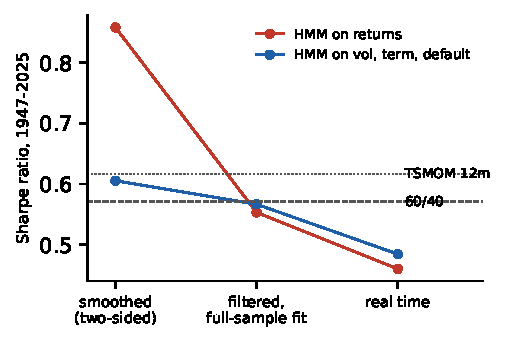
\includegraphics[width=0.9\columnwidth]{fig5_ladder}
\caption{Sharpe ratio of the same two-state HMM as its information set shrinks to what an investor knew, 1947--2025, 10 bp.}\label{fig:ladder}
\end{figure}

\section{The state of the art outside its sample}\label{sec:sjm}
We re-implemented the jump-model strategy of \citet{shu2024downside} from the paper and the authors' code: features are the exponentially weighted downside deviation (10-day halflife) and Sortino ratios (20- and 60-day halflives) of daily excess returns; features are clipped at three training standard deviations and standardised; the two-state model is refit every six months on a rolling 3,000-day window; the online state is the last state of the optimal path over the lookback; each month the jump penalty is the value in $\{0,5,15,35,70,150\}$ (the paper's grid, on its scale) whose 0/1 strategy had the highest Sharpe ratio over the preceding eight years; positions are all equity or all T-bills with a one-day delay. Applied to the CRSP market rather than the S\&P 500 index, it reproduces the paper's risk reduction on 1990--2023 (maximum drawdown $-30\%$ against $-55\%$, paper: $-26.6\%$ and $-55.2\%$) and a smaller Sharpe gain (0.51 against 0.49 at 10 bp; paper: 0.68 against 0.48). On 1950--1989, which the method never saw, it earns 0.35 against buy-and-hold's 0.59, and it does no better at 25 or 50 bp (0.38 and 0.36), because the penalty validation adapts its switching rate to cost but cannot create a premium. Before costs it would have earned 0.79: the signal is informative, but switching 6--10 times a year on it is not worth what it costs (Figure~\ref{fig:eras}).

\section{Theory: when planning matters}\label{sec:theory}
Consider a regime $s_t\in\{0,1\}$ (calm, turbulent) following a Markov chain, a signal $o_t$ whose distribution depends on $s_t$, and a finite set of portfolios $\mathcal{A}$. The investor's belief $b_t=\Pr(s_t=1\mid o_{1:t})$ is updated by the Bayes filter, a one-period utility $u_a(b)$ (e.g.\ mean-variance utility of next period's return under the predicted regime mixture) is earned, and moving from $a'$ to $a$ costs $K_{a'a}$.

\begin{proposition}[Frictionless separation]\label{prop:sep}
If $K\equiv0$ and neither the regime nor the signal depends on the action, then for every discount factor the optimal policy of the belief MDP is $a^*(b)=\arg\max_a u_a(b)$, and QMDP returns the same policy.
\end{proposition}
\emph{Proof.} The Bellman operator is $V(b)=\max_a\{u_a(b)+\beta\,\mathbb{E}[V(b')\mid b]\}$ and the continuation term does not depend on $a$; QMDP's $Q$-values differ across actions only through $u_a$. $\square$

The proposition explains a common null result: a POMDP planner built on a regime HMM collapses to the myopic rule. Planning acquires value only through a state variable the action changes. Holdings are the natural one.

\begin{proposition}[Cube-root hysteresis band]\label{prop:band}
Let the belief follow a diffusion with local standard deviation $s(b)$, let the utility gain $\Delta u(b)=u_A(b)-u_B(b)$ of a risk-on portfolio $A$ over a risk-off portfolio $B$ cross zero at $b^*$ with slope $-g<0$, and let each switch cost $K$. Under the long-run average criterion, the optimal policy holds $A$ until $b_t$ rises to $b^*+\delta$ and holds $B$ until $b_t$ falls to $b^*-\delta$, with
\begin{equation}\label{eq:law}
\delta=\left(\frac{3K\,s(b^*)^2}{2g}\right)^{1/3}\big(1+O(K^{1/3})\big).
\end{equation}
\end{proposition}
\emph{Proof sketch.} Let $x=b-b^*$ and $D=V_A-V_B$ be the difference of relative value functions inside the band; the average reward cancels. To leading order $\tfrac{s^2}{2}D''=-\Delta u=gx$ (the drift term multiplies $D'=O(\delta^2)$ and is of higher order). Value matching and smooth pasting at the two switching points, $D(\pm\delta)=\mp K$ and $D'(\pm\delta)=0$, give $D=\tfrac{g}{3s^2}x^3-\tfrac{g\delta^2}{s^2}x$, hence $D(\delta)=-\tfrac{2g\delta^3}{3s^2}=-K$. $\square$

For a regime model whose signal separates the regimes at rate $\kappa$ per unit time, the Wonham filter gives $s(b)=\kappa\,b(1-b)$. A more informative model therefore needs a wider band, and the band is widest where the belief moves fastest. The same argument with a continuum of weights gives a band of half-width $(3c\,q/2\gamma\sigma^2)^{1/3}$ around the myopic weight, $q$ being the variance rate of the target weight, the regime analogue of the general small-cost result of \citet{kallsen2017general}.

\begin{corollary}[Discrete monitoring]\label{cor:disc}
If decisions are taken every $\Delta t$, the band shrinks to $\delta_{\Delta}\approx\delta-\beta^{*}s\sqrt{\Delta t}$ with $\beta^{*}=-\zeta(\tfrac12)/\sqrt{2\pi}\approx0.5826$, and it vanishes, so that the myopic rule is optimal, when $K<K_{\min}=\tfrac{2g}{3s^2}(\beta^{*}s\sqrt{\Delta t})^3$.
\end{corollary}
The correction is the expected overshoot of a discretely sampled random walk over a barrier \cite{siegmund1979corrected}, the same constant that corrects discretely monitored barrier options \cite{broadie1997continuity}.

\textbf{Verification.} We solve the belief MDP exactly by relative value iteration on a 1,201-point belief grid with a Gauss--Hermite belief kernel, for a two-regime model refined in time ($\Delta t=1,\tfrac14,\tfrac1{16},\tfrac1{64}$, with switching hazard, drift and variance $\propto\Delta t$ and signal separation $\propto\sqrt{\Delta t}$). The exact half-width converges to (\ref{eq:law}) as $\Delta t\to0$ (ratio 0.69, 0.85, 0.93, 0.97 at $c=10^{-4}$), and at every $\Delta t$ the corrected law matches it within 2.1\% (Figure~\ref{fig:theory}).

\begin{figure}[t]
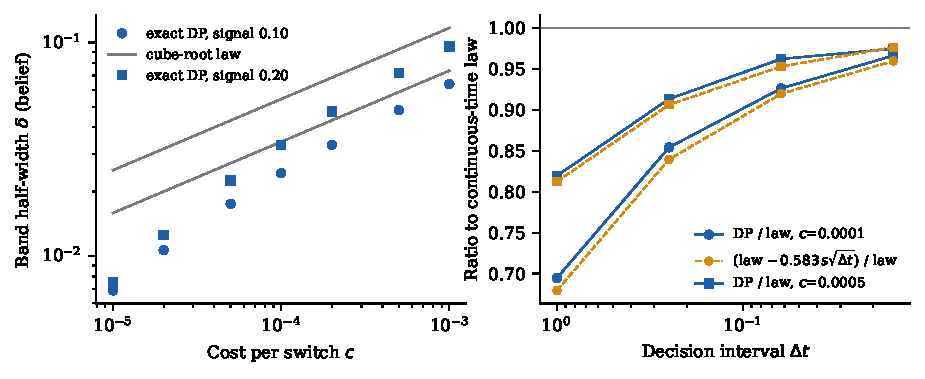
\includegraphics[width=\columnwidth]{fig2_theory}
\caption{Left: exact dynamic-programming band half-width against the cube-root law. Right: convergence of the exact band to the law as the decision interval shrinks (blue), and the discrete-monitoring correction (orange).}\label{fig:theory}
\end{figure}

\section{Planned regime timing}\label{sec:band}
We apply Proposition~\ref{prop:band} to the daily regime model that \citet{shu2024downside} use as their benchmark: a two-state Gaussian HMM on daily excess returns, refit every six months on 3,000 days, with the same one-day delay. At each refit we compute the belief kernel implied by the fitted HMM and the regime-conditional moments of returns, and solve the cost-aware belief MDP exactly (401-point grid, ten-year planning horizon, risk aversion 2). The \emph{myopic} policy acts on the same belief and utility with costs ignored; the \emph{band} policy is the DP solution. Nothing is tuned on outcomes.

Table~\ref{tab:band}, Figure~\ref{fig:wealth} and Figure~\ref{fig:costs} report 1942--2025. Myopic execution switches 13 times a year regardless of cost; its Sharpe ratio falls from 0.54 at 5 bp to $-0.01$ at 50 bp, and under historical costs it loses 94\% from peak. The band trades 3--8 times a year, falling as costs rise as the theory prescribes, and keeps a Sharpe ratio between 0.48 and 0.55 across every cost level, including historical costs. Its advantage over myopic execution is significant from 25 bp up ($p<0.001$). It is statistically indistinguishable from the jump model (band minus jump model 0.02--0.06, $p>0.5$), better before 1990 and worse in the jump model's own window. Against buy-and-hold it gives up 0.04--0.09 of Sharpe ratio (not significant) and cuts the maximum drawdown from $-50\%$ to between $-22\%$ and $-36\%$; for a CRRA investor with risk aversion 10 its certainty equivalent is 1.0--3.2\% a year against roughly zero for buy-and-hold. None of the daily strategies has a significant alpha on the market (band: 0.4\% a year, $t=0.46$).

\begin{table}[t]
\caption{Daily US equity timing, 1942--2025, monthly-compounded statistics. Sharpe ratio (SR), maximum drawdown (MDD), switches per year, and the band's Sharpe advantage with its bootstrap $p$-value.}\label{tab:band}
\small
\begin{tabular}{llrrrr}
\toprule
Cost & Strategy & SR & MDD & Sw/yr & $\Delta$SR ($p$)\\
\midrule
10 bp & Belief band & 0.48 & $-25\%$ & 6.2 & \\
 & Myopic HMM & 0.45 & $-32\%$ & 13.2 & 0.03 (0.36)\\
 & Jump model & 0.45 & $-25\%$ & & 0.03 (0.78)\\
 & Buy and hold & 0.57 & $-50\%$ & & $-0.09$ (0.20)\\
\midrule
50 bp & Belief band & 0.48 & $-34\%$ & 2.9 & \\
 & Myopic HMM & $-0.01$ & $-51\%$ & 13.2 & 0.49 ($<$0.001)\\
 & Jump model & 0.45 & $-26\%$ & & 0.04 (0.70)\\
\midrule
Historical & Belief band & 0.48 & $-36\%$ & 2.8 & \\
 & Myopic HMM & $-0.11$ & $-94\%$ & 13.2 & 0.59 ($<$0.001)\\
 & Jump model & 0.47 & $-25\%$ & & 0.02 (0.87)\\
 & Buy and hold & 0.57 & $-50\%$ & & $-0.09$ (0.20)\\
\bottomrule
\end{tabular}
\end{table}

\begin{figure}[t]
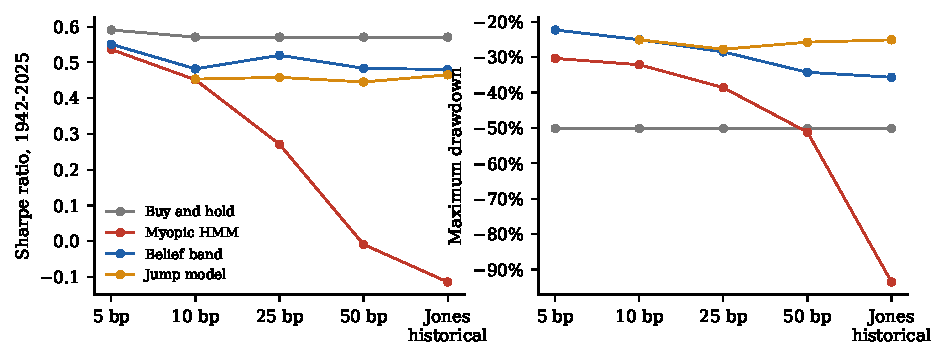
\includegraphics[width=\columnwidth]{fig3_cost_curves}
\caption{Sharpe ratio and maximum drawdown against the one-way cost, 1942--2025. Myopic execution decays with cost; the band does not.}\label{fig:costs}
\end{figure}

\begin{figure*}[t]
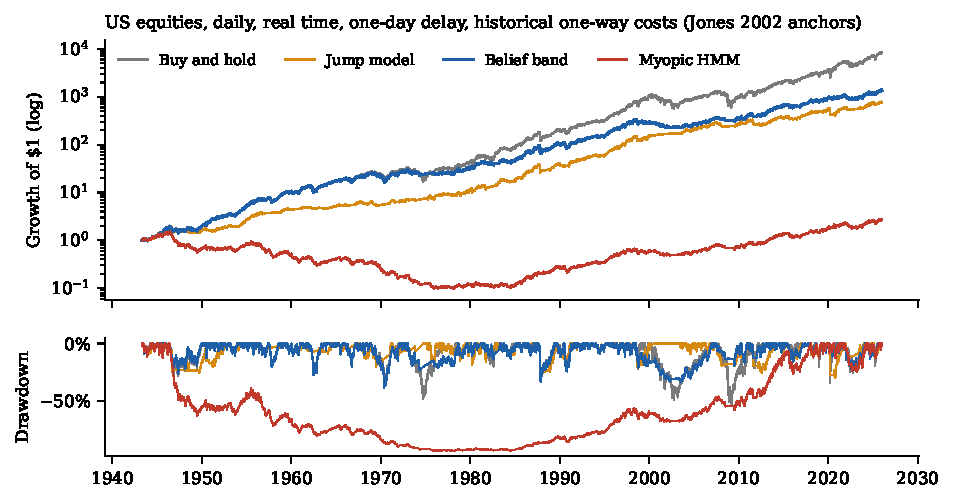
\includegraphics[width=\textwidth]{fig1_wealth_jones}
\caption{Growth of \$1 and drawdowns, daily US equities 1942--2025, real time, one-day delay, historical costs. The same HMM belief drives the myopic and band policies.}\label{fig:wealth}
\end{figure*}

Figure~\ref{fig:zoom} shows the mechanism in 2007--2010 and 2019--2021: the belief spends long stretches near the myopic threshold, where the myopic rule flips back and forth and pays each time, while the band holds its position until the evidence is strong.

\begin{figure*}[t]
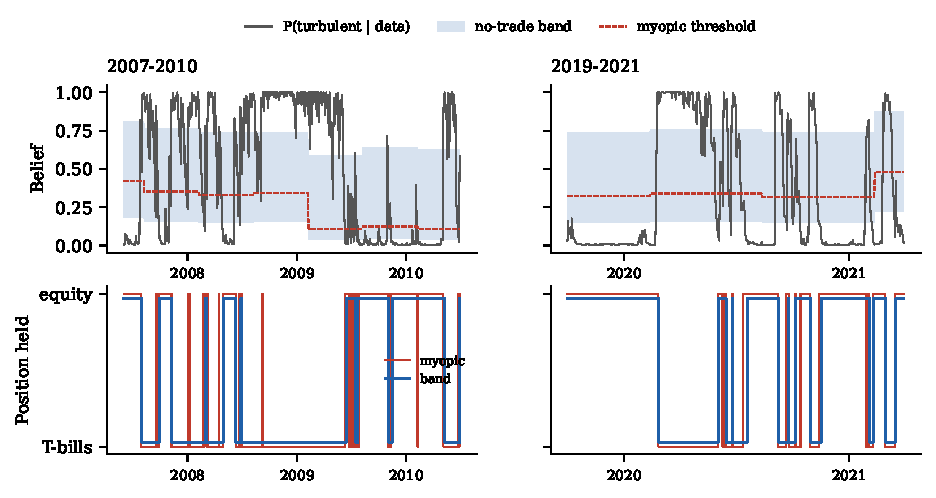
\includegraphics[width=\textwidth]{fig4_zooms}
\caption{Filtered probability of the turbulent regime, the no-trade band and the myopic threshold (top), and the positions of the two policies (bottom), at 25 bp.}\label{fig:zoom}
\end{figure*}

\textbf{Does the theory describe the bands the solver chose?} Each of the 186 refits records the belief diffusion $s^2$ at the indifference point and the slope $g$ of the utility gain. At 25 bp the median exact half-width is 0.321 and the median corrected law is 0.321 (ratio 0.97); the uncorrected law overstates it by 30\%, because daily HMM beliefs move 0.23 per day near the threshold. Under historical costs, where the cost varies across refits, the exact and predicted half-widths have a correlation of 0.93.

\textbf{Robustness.} Five position levels instead of two, planning horizons of two or thirty years, and risk aversion of 5 change the band's Sharpe ratio (computed from daily returns) by at most 0.06 and leave the myopic rule's collapse intact: at historical costs the band earns 0.54--0.58 in every variant, the myopic rule between $-0.27$ and $-0.14$ with drawdowns of 94--96\%.

\textbf{Outside the United States.} We run the jump model, the myopic HMM and the band, unchanged, on daily market excess returns for Europe, Japan, Asia-Pacific ex Japan and developed ex US (Table~\ref{tab:intl}). The common window starts when the jump model's eight-year validation first becomes available, October 2009. In this long expansion every regime strategy trails buy-and-hold by 0.2--0.4 of Sharpe ratio. The band is ahead of the jump model in six of the eight market-cost cells, and the jump model's Sharpe ratio is at or below 0.10 in seven of them.

\begin{table}[t]
\caption{Four developed markets, Oct 2009--Aug 2026, daily Sharpe ratios.}\label{tab:intl}
\small
\begin{tabular}{llrrrr}
\toprule
Market & Cost & Jump & Myopic & Band & Buy \& hold\\
\midrule
Europe & 10 bp & 0.00 & 0.07 & 0.15 & 0.42\\
 & 25 bp & $-0.02$ & $-0.05$ & 0.05 & 0.42\\
Japan & 10 bp & 0.08 & 0.30 & 0.27 & 0.43\\
 & 25 bp & 0.09 & 0.16 & 0.24 & 0.43\\
Asia-Pac.\ ex JP & 10 bp & 0.09 & 0.21 & 0.17 & 0.40\\
 & 25 bp & 0.07 & 0.08 & 0.20 & 0.40\\
Dev.\ ex US & 10 bp & 0.23 & 0.27 & 0.18 & 0.49\\
 & 25 bp & 0.10 & 0.13 & 0.14 & 0.49\\
\bottomrule
\end{tabular}
\end{table}

\begin{figure}[t]
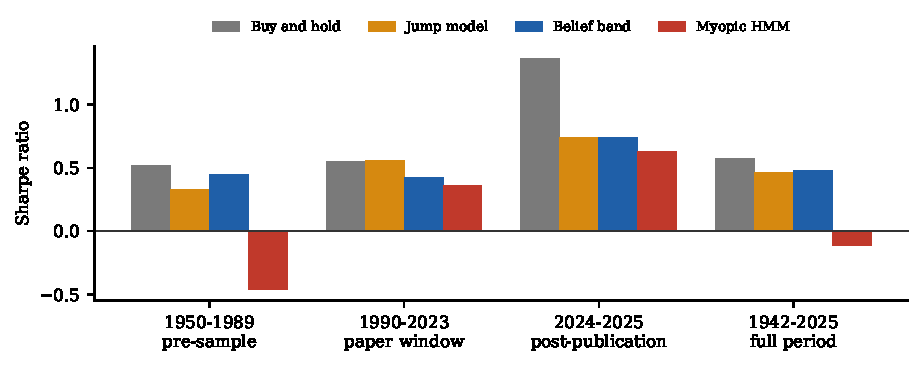
\includegraphics[width=\columnwidth]{fig6_eras}
\caption{Sharpe ratios by era under historical costs. The jump model leads only in the window it was developed on.}\label{fig:eras}
\end{figure}

\section{Implications for allocators}\label{sec:allocators}
The band is set by the cost of the instrument used to act, so the same regime view implies very different behaviour across a portfolio. Table~\ref{tab:alloc} solves the exact belief MDP for the daily equity regime signal (a model fit on the 3,000 days to 2004, near the median refit) at the one-way cost of instruments an allocator might trade on it, and counts switches along the real-time belief path of 1942--2025. Futures and ETFs are cheap enough that the band nearly vanishes and the myopic rule is close to optimal, as Corollary~\ref{cor:disc} predicts below about 0.7 bp. Treasuries, institutional equity and corporate bonds sit inside the cube-root regime: the band widens from a few hundredths to most of the belief range, and switching falls from ten to three times a year. At the discounts at which private-equity fund interests trade in the secondary market, the solution is degenerate: the optimal policy never sells, whatever the belief.

This is the logic of the denominator effect. When public markets fall, an allocator's private-equity share rises above target; restoring it means selling at secondary prices that were 54\% of NAV on average in 2009 \cite{nadauld2019liquidity} and 92\% for buyout interests in 2025 \cite{jefferies2026secondary}. Proposition~\ref{prop:band} says the tolerated deviation should scale with the cube root of that cost, which is far wider than any policy range. Raising targets, as large US public plans did in 2009 \cite{meerkatt2009shakeout}, is the band at work, not a failure of discipline. For a committee, the practical rule is to set rebalancing and tactical ranges per asset class in proportion to $(\text{cost}\times\text{signal volatility}^2/\text{utility slope})^{1/3}$, and to act on regime views through the cheapest instrument available, which for most illiquid exposure means overlays rather than sales.

\begin{table}[t]
\caption{Exact belief bands for the daily equity regime signal at asset-class trading costs (myopic threshold 0.50).}\label{tab:alloc}
\small
\begin{tabular}{lrrr}
\toprule
Instrument (source of cost) & One-way & Hold equity & Sw/yr\\
 & cost & while belief in & \\
\midrule
E-mini futures, one tick \cite{fett2017liquidity} & 0.2 bp & $\approx$0.50 (myopic) & 10.8\\
10-yr Treasury \cite{adrian2023evolution} & 0.9 bp & $[0.46, 0.57]$ & 9.5\\
Large-cap equity \cite{frazzini2018trading} & 8.9 bp & $[0.32, 0.76]$ & 5.9\\
IG corporates \cite{bessembinder2018capital,bessembinder2020survey} & 38 bp & $[0.17, 0.89]$ & 4.1\\
HY corporates \cite{bessembinder2018capital} & 51 bp & $[0.14, 0.91]$ & 3.8\\
US equity 1953--75 \cite{jones2002century} & 100 bp & $[0.08, 0.96]$ & 3.0\\
Buyout stake, 2025 \cite{jefferies2026secondary} & 8\% & never sells & 0\\
Any PE stake, 2009 \cite{nadauld2019liquidity} & 46\% & never sells & 0\\
\bottomrule
\end{tabular}
\end{table}

\section{Limitations}
Our daily study covers one regime model family on equities against T-bills; richer state spaces (three or more regimes, several assets) require belief grids on a simplex, which our solver supports but we have not run at daily frequency. The historical cost schedule interpolates between documented anchors and assumes bond costs at half of equity costs. The theory is leading-order in the cost and assumes a smooth belief diffusion near the indifference point; daily HMM beliefs jump, which is exactly why the discrete correction matters. Real-time data revisions do not affect the market-price inputs we use.

\section{Conclusion}
Over a century of real-time data, regime timing does not beat a static allocation on risk-adjusted return, and the strongest published results depend on information or sample choices an investor did not have. What regime signals can do is reduce drawdowns, and only if the trading rule accounts for the cost of acting on uncertain beliefs. The frictionless POMDP gives no reason to plan; the costly one gives a band whose width follows a cube-root law. Executed through it, a regime signal that destroys capital under myopic switching becomes a drawdown control that is competitive with the best published method, across eras, costs and markets.

\bibliographystyle{ACM-Reference-Format}
\bibliography{refs}
\end{document}
